\chapter{Méthodologie}
\minitoc%

\section{Données Fonctionnelles : l'essentiel}

    \subsection{Définitions et propritétés informelles}


Commençons par introduire les données fonctionnelles de manière informelle afin de mieux intégrer la définition formelle, plus utile pour la manipulation.

Cette section regroupe l'ensemble des messages essentiels à retenir des données fonctionnelles pour la pratique, sans alourdir les notions avec des notations mathématiques. Le cadre formel sera traité juste après.

\begin{definition*}[données fonctionnelles — informel]
    Les données fonctionnelles sont des données dont les observations sont des fonctions, c'est-à-dire des courbes, des surfaces, des images, \, \dots
    
    i.e : toute donnée ayant une dépendance de type "relation fonctionnelle" avec un ou plusieurs paramètres.
    \label{def*:fda}
\end{definition*}

\begin{figure}[H]
    \begin{center}
        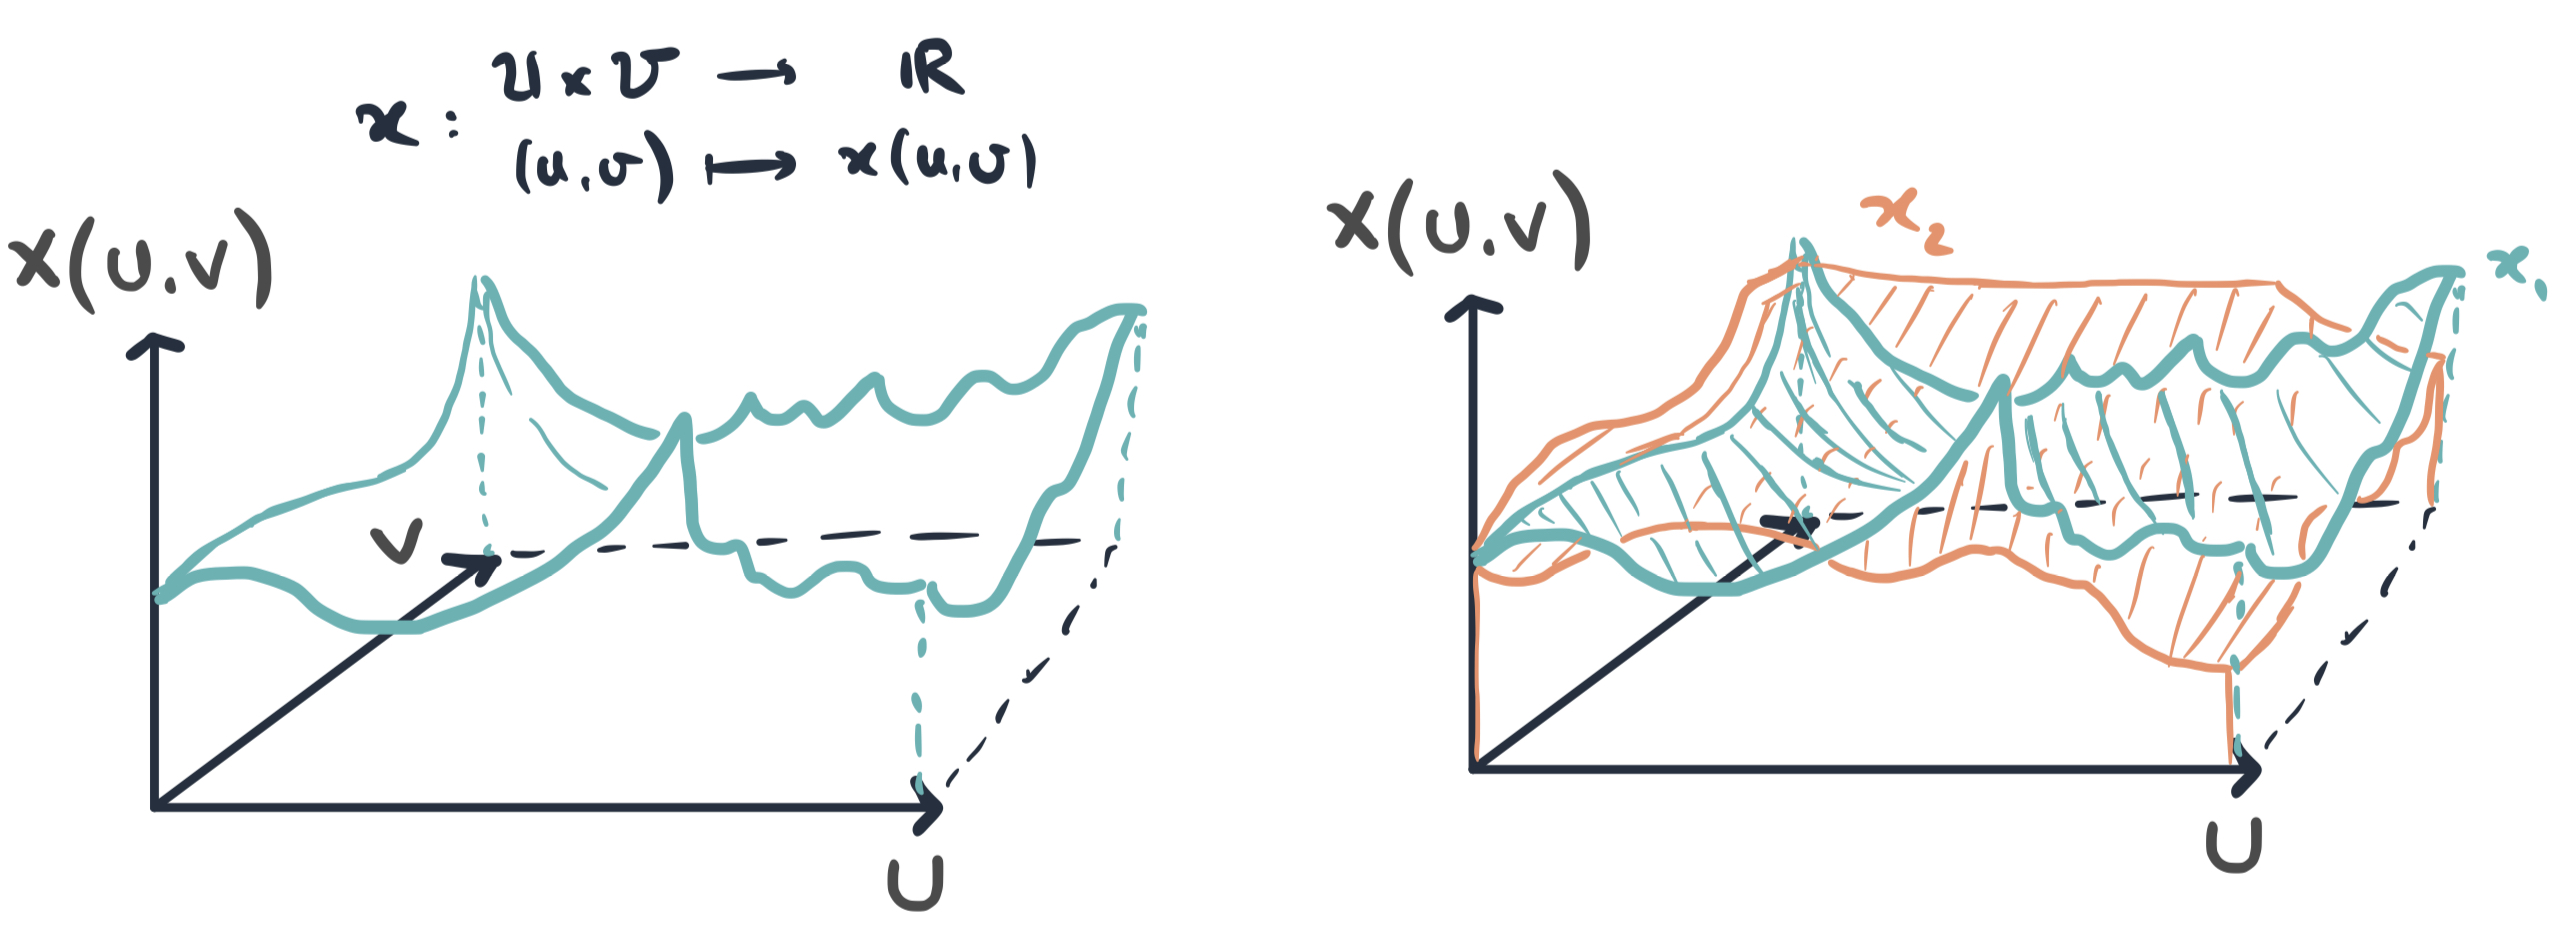
\includegraphics[width=\textwidth]{Images/sketches/fda_surface.jpg}
    \end{center}
    
    {
    \textbf{Gauche :} exemple de surface
    \\
    \textbf{Droite :} échantillon de deux observations de la surface suivant une loi fonctionnelle}

    \caption{Donnée fonctionnelle : relation fonctionnelle avec plusieurs paramètres}
    \label{fig:sketch_surface}
\end{figure}

Maintenant introduites, les théorèmes suivant permettent de manipuler ces données à la fois pour la théorie et la pratique :

\begin{thm*}[\nameref{thm:KL} — informel]
    \noindent\fbox{%
    \parbox{\textwidth}{%
    Il est possible pour une large classe de données fonctionnelles de les décomposer dans une base \emph{de fonctions} adaptée aux données (au sens de la covariance) que l'on appelle base ACP fonctionelle (FPCA).
    }%
    }
    \label{thm*:KL}
\end{thm*}
\begin{proof}[\faCogs \, preuve informelle]
    La covariance est un opérateur bilinéaire symétrique défini positif, on peut donc appliquer le théorème de Mercer (équivalent du théorème spectral) qui nous donne une base orthonormale de $\mathds L^2$ sur laquelle on va décomposer notre processus \textbf{centré}.
\end{proof}
\begin{rem}
    La classe de fonctions pouvant être décomposées est large, puisqu'elle regroupe l'ensemble des processus qui nous intéressent la plus part du temps en tant que statisticien : celles qui sont à support sur un intervalle, admettant une covariance continue et finie sur le support.
\end{rem}
    
On en déduit que pour travailler avec des données fonctionnelles, il suffit de les décomposer dans la base ACP fonctionnelle puis de travailler sur les composantes de chaque élément de la base. On travaille désormais avec des réels et non plus des fonctions, ce qu'on aime manipuler. On peut alors faire de la statistique traditionnelle avec les outils que l'on connait.


\begin{propriete*}[intérêt de la base FPCA — informel]
    \noindent\fbox{%
    \parbox{\textwidth}{%
    la base ACP fonctionnelle est la plus économe, c'est à dire qu'elle explique au mieux la covariance des données pour un nombre de composantes fixées, ce qui est utile car on ne sait manipuler numériquement que des objets de dimension finie.
    }%
    }
\end{propriete*}

\subsection{estimation adaptative informelle}

On a mentionné qu'il serait judicieux de lisser les observations en tenant compte de la régularité du processus dont est issu nos données. La question est désormais la suivante :

\question{
    Est-il possible de récupérer la régularité locale des trajectoires à partir des données ? Si oui, comment ?
}

C'est ce qu'affirme le théorème suivant à partir des travaux de Golovkine et al. ainsi que Maissoro-Patilea-Vimond (MPV) :

\begin{thm*}[Regularité locale — informel]
    \noindent\fbox{%
    \parbox{\textwidth}{%
    Les données fonctionnelles permettent de récupérer la régularité locale des trajectoires. Les estimateurs définis \textbf{ponctuellement} convergent. 
    }%
    }
    \label{thm*:regularite_locale}
\end{thm*}
\begin{rem}[Continuité de Kolmogorov]
    Un théorème (\nameref{thm:kolmogorov_continuite}) permet à partir de l'espérance d'incréments d'un processus aléatoire de déduire sa régularité.
    C'est pourquoi les estimateurs sont définis à partir de l'espérance des incréments quadratiques du processus. C'est entre autres \emph{la raison pour laquelle les données fonctionnelles permettent de récupérer la régularité locale des trajectoires}.

    \label{rem:kolmo_continuite}
\end{rem}

Les motivations de l'obtention de la régularité étaient en partie de pouvoir mieux estimer les quantités qui nous intéressent dont la fonction moyenne du processus, ainsi que son opérateur de covariance. Ce qui est à la fois important pour l'analyse (via l'interprétation de la base ACP déterminée par la covariance) et pour la prédiction. On peut alors se demander si il existe des estimateurs de la moyenne et de la covariance prenant en compte la régularité locale. C'est ce qu'affirme les théorèmes suivants :

\warn{demander à Hassan la dernière version de son papier car la partie d estimation adaptative a beaucoup changé}

\begin{thm*}[Estimateurs de la moyenne et de la covariance — informel ~\cite{golovkine2021adaptive}]
    \noindent\fbox{%
    \parbox{\textwidth}{%
    Il est possible en lissant les observations par méthode à noyaux avec une largeur de bande \emph{spécifique à l'objet que l'on souhaite estimer}, de dériver des estimateurs de la moyenne et de la covariance qui convergent. 
    La largeur de bande optimale \emph{pour l'objet que l'on souhaite estimer} est celle qui minimise un risque qui effectue un compromis biais-variance, qui dépend de la régularité locale du processus, en pénalisant les largeurs de bande menant à des "trous" dans les fonctions lissées.
    On parle d'\emph{\og estimation adaptative \fg}.
    }%
    }

    \label{thm*:estimation_adaptative}
\end{thm*}

Cependant, bien qu'une largeur de bande optimale existe, elle est inconnue. Il est donc important de savoir si le praticien peut l'estimer, et avec quelle précision (c'est à dire à quel point l'estimateur sera biaisé ou non). C'est ce que nous affirme le théorème suivant :

\pagebreak

\begin{thm*}[expression de la largeur de bande optimale — informel ~\cite{golovkine2021adaptive}]
    \noindent\fbox{%
    \parbox{\textwidth}{%
    Sous certaines hypothèses de régularité du processus, et d'indépendance des temps observés, la largeur de bande optimale peut être approchée (avec forte probabilité de bonne approximation) par une expression ne dépendant que du nombre de courbes observées, du nombre moyen de temps observés par courbe, et de la régularité locale du processus. Ce biais de l'estimateur de la fonction moyenne est alors contrôlé en fonction de ces mêmes quantités.

    Sous des hypothèses un peu plus fortes sur le nombre d'observations par courbe, et le nombre de courbe on dispose de résultats similaires pour l'estimateur de la covariance.}%
    }
        
    \label{thm*:h_opt_estim}
\end{thm*}


Enfin, on peut se demander ce qu'il en est des estimateurs dans le cadre où l'on dispose de la dépendance dans les données (ce qui est la cas pour les données éoliennes notamment). Ce cas est traîté par le théorème suivant dérivé par MPV :

\begin{thm*}[ Estimation adaptative de séries temporelles fonctionnelles — informel ~\cite{maissoro-SmoothnessFTSweakDep} ]

    On peut estimer la régularité d'une série temporelle de données fonctionnelles à condition que la mémoire temporelle de la série soit courte. (La décroissance de la dépendance temporelle doit être au moins aussi rapide qu'une décroissance géométrique)

    \label{thm*:far_adaptative_estimation}
\end{thm*}

\pagebreak

\subsection{Résumé informel de la méthodologie}

Les données fonctionnelles permettent de travailler sur un modèle où la \emph{relation} entre plusieurs quantités est sujet à une loi \colorize[flatuicolors_biscay]{[$cf$ \nameref{def*:fda}]}. Ce point de vue de réplication de courbes est notamment utile car il permet d'extraire des observations leur régularité \colorize[flatuicolors_biscay]{[$cf$ \nameref{rem:kolmo_continuite}, \nameref{thm*:regularite_locale}]}. L'estimation de cette régularité permet, entre autres, de lisser les courbes de façon appropriée en fonction de la quantité que l'on souhaite estimer, telle que la moyenne et la covariance avec une plus grande précision \colorize[flatuicolors_biscay]{[$cf$ \nameref{thm*:estimation_adaptative}]}. 

\noindent\begin{figure}[H]
    \centering
    \pagewidthimg{Images/sketches/sketch_resume_informel.jpg}
    \caption{Résumé des motivations du de l'estimation de la régularité locale des trajectoires}
    \label{fig:sketch_resume_informel}
\end{figure}


\pagebreak

\subsection{Données fonctionnelles : formellement}

\subsubsection{Définition formelle}

Pour éviter d'alourdir les notations, on se place dans le cas où les fonctions sont à valeurs dans $\mathds R$ et à support sur un intervalle fermé $I$ de $\mathds R$. Toutefois, on peut très bien considérer des fonctions à valeurs dans $\mathds R^d$ et à support sur un compact $K$ de $\mathds R^p$ sans perte de généralités.

\begin{definition}[données fonctionnelles ]

    On appelle données fonctionnelles, un échantillon $\famfinie x 1 n$ de fonctions continues $x_i : I \rightarrow \R d$ issues d'un processus $X$ défini comme ci-dessous :

    $$X : 
    \begin{array}{ccc}
        \Omega & \longrightarrow & \mathcal C(I, \mathds R)
        \\
        \omega & \longmapsto & X(\omega) = x 
    \end{array}
    $$

\end{definition}

\subsubsection{Résultats importants}

On énonce désormais le théorème central de l'analyse de données fonctionnelles qui n'est autre que la décomposition dans la base FPCA de notre processus.

\begin{rem}
    on notera que dans le cadre des données fonctionnelles, on ne travaille pas de façon générale avec la covariance :
    
    $$C_X : (s,t) \mapsto \esperance{ (X - \mu)(s) \cdot (X - \mu)(t) }$$
    
    On travaille plutôt avec l'\textbf{opérateur} de covariance :
    $$f \mapsto \int\limits_I f(u)C_X(u, \cdot \,) \,du$$ 
    
    C'est parceque cet opérateur est linéaire continu (car Hilbert-Schmidt donc borné pour la norme d'opérateur) symétrique semi-défini positif (pour le produit scalaire de $\mathds L^2$) et que l'on peut donc en faire une décomposition spectrale sur une base orthonormale de vecteurs propres associés à des valeurs propres positives. Cette décomposition est à la base des approximations que le praticien effectuera ainsi qu'à la base de la dérivation de nombreux théorèmes et propriétés.
\end{rem}

\bigskip

Etant donné que l'on traîte des données fonctionnelles, on considère la géométrie usuelle de $\mathds L^2(\mathds R, \, \lambda)$ et on note ainsi 

$$\prodscalselon \cdot \cdot {\mathds L^2}: \begin{array}{ccc}
    \mathds L^2 \times \mathds L^2 & \longrightarrow & \mathds R
    \\
    (f,g) & \longmapsto & \int f(u)g(u) \, d\lambda(u) 
\end{array}$$ 

le produit scalaire que l'on considère pour manipuler les données fonctionnelles.

% https://stackoverflow.com/a/4008463 : no page break
\begin{minipage}{\textwidth}
\begin{thm}[Karhunen-Loeve]
    \emph{référence :} ~\cite[pages : 238-239-241]{kokoszka2017introduction}

    \textbf{Hypothèses :}

    $$
    \boxed{
    \begin{array}{ll}
        \textsf{\faCaretSquareRight} & X \in \mathds L^2( \Omega, \mathcal C(I, \mathds R)) 
        \\ \\
        \textsf{\faCaretSquareRight} & \textsf{covariance : } C : \begin{array}{ccc}
            \mathds L^2( \Omega, \mathcal C(I, \mathds R)) & \longrightarrow & \mathcal C(I^2, \mathds R)
            \\
            X & \longmapsto & C_X
        \end{array}
        \\ \\
        & \textsf{ie : } C_X : (s, t) \mapsto C_X(s,t) \textsf{ est continue}
        \\ \\
        \textbf{\faIcon{asterisk}} & \textsf{opérateur covariance} \, c_X[ \, \cdot \, ] : \begin{array}{ccc}
            \mathcal C(I, \mathds R) & \longrightarrow & \mathcal C(I, \mathds R)
            \\
            f & \longmapsto & \int_I f(s) C_X(s, \cdot \, ) \, ds \end{array}
        \\\\
        \textsf{\faCaretSquareRight} & \textsf{valeurs propres ordonnées : } \forall p \geq 1, \lambda_{p+1} \leq \lambda_p \quad\quad \lambda_p, \lambda_{p+1} \in \operatorname{sp}(c_X)
        \\ \\
        \textbf{\faIcon{asterisk}} & \textsf{on pose } \overrightarrow{sp}_{\orthonormal}^{[1,p]}(c_X) \isdef \left\{ \phi_k \in \overrightarrow{sp}_{\orthonormal}( \, c_X \, ) \textsf{ associé à }  \lambda_k, k \in \intervaleint 1 p \, \right\}
    \end{array} 
    }
    $$

    \textbf{alors :}
    $$
    \boxed{
    \begin{array}{cc}
        \textsf{\faCaretSquareRight} & 

            \forall p \geq 1 
            \quad
            \argmin\limits_{u_k \in \mathcal C(I, \mathds R)} \mathds E \left\Vert X - \sum\limits_{k=1}^p \prodscalselon {X - \mu} {u_k} {\mathds L^2} u_k \right\Vert^2 = \overrightarrow{sp}_{\orthonormal}^{[1,p]}( \, c_X \, )

        \\
        \\
        \textsf{\faCaretSquareRight} & X = \mu + \sum\limits_{k=1}^{+\infty} \prodscal {X - \mu} {\phi_k} \phi_k
        \\
        &
        \\
         &\textsf{avec } \phi_k \in \overrightarrow{sp}_{\orthonormal}( \, c_X \, )
    \end{array}
    }
    $$

    \label{thm:KL}
\end{thm}
\end{minipage}

\begin{rem}
    pour pouvoir ordonner les valeurs propres dans l'ordre décroissant, et sélectionner les composantes principales les plus informatives, il faut pouvoir réarranger l'ordre de la somme. Pour cela il faut que les valeurs propres forment une famille sommable, une condition suffisante et souvent utilisée est que $\mathds E \Vert X \Vert^2 < \infty$ 
\end{rem}

\begin{rem}
    la propriété de la section précédente sur l'aspect économe de la base FPCA découle directement de l'assertion $\forall p \geq 1 
    \quad
    \argmin\limits_{u_k \in \mathcal C(I, \mathds R)} \mathds E \left\Vert X - \sum\limits_{k=1}^p \prodscal {X - \mu} {u_k} u_k \right\Vert^2 = \overrightarrow{sp}_{\orthonormal}^{[1,p]}( \, c_X \, )$ dans le théorème de Karhunen-Loeve.
\end{rem}




    \subsection{Cas non indépendant : séries temporelles de données fonctionnelles}
        
    Une large partie de la théorie des données fonctionnelles suppose que l'on observe des courbes $X_i : \Omega \rightarrow \mathcal C^0(I, \mathds R)$ \textbf{indépendantes} et identiquement distribuées. Cependant une partie non négligeable des données que l'on observe ont des dépendances avec les valeurs passées. Par exemple, il est raisonnable de penser que la consommation électrique d'un foyer au cours d'une année croît avec l'ajout successif de nouveau appareils électroniques. L'hypothèse d'indépendance entre les données n'est donc plus pertinente pour les données que l'on traite et il devient important de considérer des processus autorégressifs adaptés aux données fonctionnelles. 
Si dans le cadre des données de $\mathds R$ cette relation de \emph{dépendance linéaire} avec le passé pouvait s'écrire sous la forme suivante 
$X_n = \sum\limits_{k=1}^{n-1} \varphi_k \, X_k + \varepsilon_n$ où $\varphi_k \in \grandR$ 
et 
$\varepsilon_n \begin{cases} \in \operatorname{VA}(\grandR) \\ \indep \sigma\left( X_i \right)_{1\,: \, n-1}\end{cases}$, 
dans le cadre fonctionnel on capture la même idée en considérant 
$X_n = \sum\limits_{k=1}^{n-1} \phi_k \left( X_k \right) + \varepsilon_n$ où $\phi_k$ 
est un \emph{opérateur linéaire} de $\mathds L^2(I, \mathds R)$, 
le plus souvent intégral. 

\chk{
    Il s'agit d'une généralisation naturelle de la relation dans le cadre réel, puisqu'on peut démontrer que sur l'espace des nombres réels l'ensemble des fonctions linéaires $\phi : \grandR \rightarrow \grandR$ sont de la forme $x \mapsto ax$ avec $a \in \grandR$. La relation sur $\grandR$ que l'on a vue juste avant peut alors se ré-écrire de façon similaire à la version fonctionnelle.
    }

On considère lors de ce stage des séries temporelles de données fonctionnelles car les données que l'on manipule ( en l'occurence les données de courbe de charge des parcs éoliens ) semble être naturellement corrélées dans le temps. 

\warn{Il faut cependant faire attention avec l'interprétation de séries temporelles fonctionnelles. En effet l'interprétation que l'on fait d'une série temporelle fonctionnelle ne peut être véritable calquée sur l'interprétation dans la cadre réel. 

\quad Si sur $\mathds R$ la corrélation temporelle s'interprête comme le fait que l'observation suivante (c'est à dire le facteur de charge du parc éolien) dépend de l'observation précédente (c'est à dire dépend du jour précédent par exemple), dans le cadre fonctionnel l'observation est une fonction. On rappelle que dans le cadre des données éoliennes, chaque observation est la courbe de charge observée su un an. Ce que cela signifie, c'est que la dépendance à l'observation passée que l'on va constater sur l'observation suivante n'affecte pas un unique point. Elle affecte tous les points de la courbe de charge simultanément. La dépendance temporelle concerne l'année entière, d'une année à l'autre. Fixer le $t$ dans $X_n(t)$ ne garantit pas l'observation de la même structure de dépendance comparé à la série temporelle fonctionnelle. 

\quad Par exemple, en utilisant un opérateur intégral pour $\phi_k$, comme $\phi_k :X \mapsto \int_I  \beta_k(u,t) X(u) du$, la vision de regarder les $t$ individuellement et de regarder leur évolution selon les années n'est pas évidente à interpréter car $\phi_k(X)$ intègre des informations de $X$ sur l'ensemble des $t \in I$, dû à l'intégrale.}

\pagebreak

\section{Estimation de la régularité locale des trajectoires}

\subsection{Ce qu'on entend par régularité locale}


Longtemps, il était cru que les fonctions continues étaient dérivables presque partout. C'est notamment Weierstrass qui a démontré qu'il existe des fonctions continues partout mais dérivable nulle part. Poincaré notamment disait de tels objets qu'ils n'existaient que pour contredire le travail des pères. 
Cependant, des objets manipulés tous les jours comme le monde de la finance notamment traitent des processus qui sont fondamentalement irréguliers
%
\footnote{les fonctions dérivables nulle part sont même denses dans les fonctions continues pour la topologie de la convergence uniforme~\cite{gourdon2020maths-dense-non-deriv}. A epsilon près on rencontre toujours une fonction dérivable nulle part lorsque l'on considère la distance maximale réalisée entre deux fonctions continues sur leur support $I$...}
%
(au point de vue de l'analyse, où l'on traite souvent des fonctions au moins dérivables). Il est donc important de pouvoir quantifier la régularité d'une fonction de façon plus fine que le nombre de dérivées qu'elle possède. 

Nous allons repasser rapidement en revue les différents concepts de régularité pour mettre l'emphase dans ce que l'on considère comme régularité locale.

Afin de savoir à quel niveau de régularité nous souhaitons estimer, il est important de garder en tête un ordre de différents niveaux de régularité résumé par les relations suivantes :

$$\textsf{Lipschitz} \implies \textsf{Hölder} \implies \underbracket{\colorize{\textsf{Localement Hölder}}}_{\textsf{ce qui nous intéresse}} \implies \textsf{Uniformément continue} \implies \textsf{Continue}$$

Afin de mieux discerner ce que chaque propriété signifie, et quelles sont les différences entre chaque niveau de régularité, nous allons rappeler rapidement les définitions de ces propriétés.

\begin{itemize}
    \item Continuité :
    $$(\forall \varepsilon > 0) \, (\forall x) (\exists \delta_{\colorize x} > 0) (\forall y) \, |x-y| < \delta \implies |f(x) - f(y)| < \varepsilon$$
    \item Uniforme Continuité :
    $$(\forall \varepsilon > 0) \, (\exists \delta > 0) (\forall x,y ) \, |x-y| < \delta \implies |f(x) - f(y)| < \varepsilon$$

    \item Lipschitz :
    $$\exists L_I \quad(\forall x,y \in I) \quad |f(x) - f(y)| < L_I |x-y|$$
    \item Hölder :
    $$
    \exists \alpha \in (0,1] \quad \exists L_{\alpha(I)} \quad (\forall x,y \in I) \quad |f(x) - f(y)| < L_{\alpha(I)} |x-y|^\alpha
    $$
    \brain{
    une fonction lipschitz est une fonction Holderienne avec $\alpha = 1$
    }

    \item Localement Hölder :
    $$
    \forall x_0 \in I \quad \exists \alpha\left(x_0\right), L_{\alpha(x_0)}\left( x_0\right) \quad \begin{cases}
    (\forall x) \quad |f(x) - f(x_0)| < L_{\alpha(x_0)} |x-x_0|^{\alpha(x_0)}
    \\
    \quad 0 < {\alpha(x_0)} \leq 1 
    \end{cases}
    $$
\end{itemize}

\question{
    \smallskip\centering
    Pourquoi se concentrer sur des processus localement Hölder ?
}

La nature des phénomènes rencontrés dans la vie réelle est souvent complexe. Influencés par de nombreux phénomènes, certains d'entre eux sont, comme mentionnés précédemment, irréguliers. C'est notamment le cas des courbes de charge électriques, qui dépendent de multitudes de phénomènes physiques ou comportementaux, dont on peut attendre une certaine régularité, mais qui ne sont pas nécessairement uniformes tant sur leur niveau régularité que l'intervalle de temps sur lequel ils ont une influence. On pourrait par exemple attendre une différence de régularité de la production électrique en plein été (soleil et température stables \ldots) comparé au mois de mars (plus grande instabilité des conditions climatiques).

De plus, les fonctions Hölderiennes représentent une classe suffisamment large de fonctions. 
% \editorwarn{citer le papier sur le fractional brownian motion (how large)}
L'espace de fonctions sur lequel on travail est donc devrait être en pratique suffisamment grand pour inclure l'ensemble des processus qui nous intéressent. Enfin les fonctions que le praticien sera amené à manipuler seront des fonctions d'un intervalle dans $\mathds R$, qui lorsque continues sont automatiquement uniformément continues en vertu du théorème de Heine. Il est donc naturel de se concentrer sur des fonctions localement Hölderiennes. \footnote{Afin de ne pas alourdir l'essence du propos, une simplification par rapport à l'article de MPV~\cite{maissoro-SmoothnessFTSweakDep} a été faite, si le lecteur souhaite aller dans le détail, il est possible de se référer à l'Annexe \ref{annexe:regularite-locale}.}


\subsection{Estimation des paramètres régularité locale des trajectoire}

\subsubsection{Deux méthodes d'obtention de la régularité locale des trajectoires}

Il existe deux méthodes différentes pour estimer la régularité des trajectoires. Si la clé des deux méthodes pour extraire la régularité locale est le théorème de continuité de Kolmogorov énoncé ci-dessous, les deux méthodes diffèrent par les points $t \in \mathcal T$ considérés dans l'estimation des accroissements quadratiques $\esperance{ \vert X(u) - X(v) \vert^2 }$ utilisés pour l'estimation de la régularité locale. 

\begin{thm}[Continuité de Kolmogorov]
    \emph{référence : } ~\cite[thm : 2.197 | page : 145]{capasso2015introduction}

    $$
    \begin{array}{ll}
        \textsf{\faCaretSquareRight} 
        & X : \, \begin{array}{ccc}
            \mathbb{R_+} \times \Omega & \longrightarrow & \mathbb{R} \\
            (t, \omega) & \longmapsto & X(t, \omega) = x(t)
            \end{array} \textsf{séparable}
        & &
        \\
        \textsf{\faCaretSquareRight}
        & \exists r,c, \varepsilon, \delta \in \mathds R_+ \quad (\forall h < \delta)(\forall t \in \mathds R_+)  \quad \esperance{ | X(t+h) - X(t) |^r } \leq c\cdot h^{1+\varepsilon}
    \end{array}
    $$
    \begin{center}
        $\Downarrow$
    \end{center}
    $$ 
    \textbf{\faIcon{asterisk}}\, \boxed{
        X \textsf{ est continu en } t \in \mathds R_+ \textsf{ pour presque tout } \omega \in \Omega
    }
    $$
    \begin{center}
        ie : il existe une version $\tilde X$ de $X$ continue en $t$ telle que $\proba{ \tilde X(t) = X(t)} = 1$
    \end{center}

    $$
    \textbf{\faIcon{asterisk}} \, \boxed{
        \tilde{X} \textsf{ est } \gamma \textsf{-Hölderienne en } t  \textsf{ pour tout } 0 < \gamma < \frac{\varepsilon}{r}
    }
    $$
    \label{thm:kolmogorov_continuite}
\end{thm}

Etant donné que notre estimateur utilise les incréments quadratiques, on se place dans le cas où $r = 2$.

% \editorwarn{Mettre la version avec Hölder, qui permet de dériver des fda la régularité locale}


La méthode de Golovkine et al. ~\cite[pages : 7—9]{golovkineRegularityOnlineEstimationNoisyCurve} n'utilise que les points observés, et construit un estimateur des incréments quadratiques à base de statistique d'ordre. 

$$\theta( T_{(l)}, T_{(k)}) = \esperance{ \left| X( T_{(l)}) - X(T_{(k)}) \right|^2 }  \begin{align*}
    &\quad \underset {\textsf{LGN}} \approx 
    & \boxed{\frac 1 {N} \sum\limits_{n=1}^N \left| \statrang Y n {2k-1} \statrang Y n k \right|^2 \isdef \hat \theta_k}
    \\
    & \, \underset {+ \mathcal C^0 Kol.} {\overset {\textsf{Hölder}} \approx}
    & L_{t_0} \esperance{| \ordered T l - \ordered T k |^{2H_{t_0}}} 
    & \rightarrow H_{t_0} = f(\theta)
\end{align*}  $$

$$\hat H_{t_0}(k) = \begin{cases} \displaystyle\frac{\log\left( \hat \theta_{4k-3} - \hat \theta_{2k-1}  \right) - \log \left(  \hat\theta_{2k-1} - \hat \theta_k \right)}{2\log 2} & \hat \theta_{4k-3} > \hat \theta_{2k-1} > \hat \theta_{k}
    \\
    1 & \textsf{sinon}
\end{cases}$$

\info{Cette méthode peut s'avérer spécifiquement utile lorsque l'on traite un flux de données, car l'arrivée de nouvelles données ne nécessite pas spécifiquement de recalculer les incréments quadratiques sur l'ensemble des points observés. }

L'autre méthode proposée par ~\cite{golovkine2021adaptive,maissoro-SmoothnessFTSweakDep}, elle se base sur l'utilisation de points non observés, inférés par lissage des courbes, à une distance $\Delta / 2$ les uns des autres pour estimer les incréments quadratiques. Cette dernière méthode implique le choix d'un hyper-paramètre lors de l'estimation $\Delta$ et pourrait être sensible à la qualité du lissage de la courbe. Etant donné que l'objectif de la détermination de la régularité locale est de pouvoir faire un lissage à noyaux adaptatif en fonction de l'objet que l'on souhaite estimer, on appelle le lissage effectué pour estimer la régularité \og pré-lissage \fg.

% https://tex.stackexchange.com/questions/156993/plotting-weierstrass-function
\begin{figure}[H]
    \centering
    \begin{minipage}{0.45\linewidth}
        \begin{tikzpicture}
    \pgfmathsetmacro{\pgfdeltavalue}{0.25}
    \pgfmathsetmacro{\pgftvalue}{0.4}
    \pgfmathsetmacro{\pgfarrowheight}{-0.25}
    \pgfmathsetmacro{\pgfarrowfrom}{\pgftvalue - \pgfdeltavalue/2}
    \pgfmathsetmacro{\pgfarrowto}{\pgftvalue + \pgfdeltavalue/2}
    \begin{axis}[axis lines=middle,
        xmin=0, xmax=1,
        ymin=-0.4, ymax=0.4,
        axis equal image,
        ytick=\empty,
        xtick=\empty,
    ]
    \addplot [flatuicolors_green, samples=300, domain=0:1.1] {weierstrass(2*x,2,15)};

    \addplot [flatuicolors_imperial, mark=*, only marks] coordinates {(\pgftvalue, {weierstrass(2*\pgftvalue,2,15)})};
    \addplot [flatuicolors_imperial, mark=*, only marks] coordinates {(\pgftvalue - \pgfdeltavalue/2, {weierstrass(2*(\pgftvalue - \pgfdeltavalue/2),2,15)})};
    \addplot [flatuicolors_imperial, mark=*, only marks] coordinates {(\pgftvalue + \pgfdeltavalue/2, {weierstrass(2*( \pgftvalue + \pgfdeltavalue/2 ),2,15)})};

    \addplot[color=flatuicolors_imperial,mark=none, thick, dashed] (\pgftvalue + \pgfdeltavalue/2,x);
    \addplot[color=flatuicolors_imperial,mark=none, thick, dashed] (\pgftvalue - \pgfdeltavalue/2,x);
    \addplot[color=flatuicolors_imperial,mark=none, thick, dashed] (\pgftvalue,x);

    \draw[color=white, fill=white] (\pgftvalue - 0.005, \pgfarrowheight - 0.05 - 0.025) rectangle (\pgftvalue + 0.005, \pgfarrowheight - 0.05 + 0.025);
    \node at (axis cs: \pgftvalue, \pgfarrowheight - 0.05) {$\colorize[flatuicolors_aqua]{ \mathbf \Delta}$};

    \draw[flatuicolors_aqua, ->] (axis cs:\pgfarrowfrom, \pgfarrowheight) -- (axis cs: \pgfarrowto, \pgfarrowheight);
    \draw[flatuicolors_aqua, <-] (axis cs:\pgfarrowfrom, \pgfarrowheight) -- (axis cs: \pgfarrowto, \pgfarrowheight);
        
    \draw[color=white, fill=white] (\pgftvalue - 0.05, -0.06) rectangle (\pgftvalue + 0.05,-0.005);
    \node at (axis cs: \pgftvalue,  -0.03 ) {$\colorize[flatuicolors_imperial]{ t_2}$};
    \draw[color=white, fill=white] (\pgftvalue - \pgfdeltavalue/2 - 0.05, -0.06) rectangle (\pgftvalue - \pgfdeltavalue/2 + 0.05,-0.005);
    \node at (axis cs: \pgftvalue - \pgfdeltavalue/2 -0.01,- 0.03) {$\colorize[flatuicolors_imperial]{ t_1}$};
    \draw[color=white, fill=white] (\pgftvalue + \pgfdeltavalue/2 - 0.005, 0.005) rectangle (\pgftvalue + \pgfdeltavalue/2 + 0.005, 0.08);
    \node at (axis cs: \pgftvalue + \pgfdeltavalue/2, 0.04 ) {$\colorize[flatuicolors_imperial]{ t_3}$};
    
    \end{axis}

\end{tikzpicture}

    \end{minipage}
    \hfill
    \begin{minipage}{0.45\linewidth}
        \begin{tikzpicture}
    \pgfmathsetmacro{\pgfdeltavalue}{0.25}
    \pgfmathsetmacro{\pgftvalue}{0.15}
    \pgfmathsetmacro{\pgfarrowheight}{-0.25}
    \pgfmathsetmacro{\pgfarrowfrom}{\pgftvalue - \pgfdeltavalue/2}
    \pgfmathsetmacro{\pgfarrowto}{\pgftvalue + \pgfdeltavalue/2}
    \begin{axis}[axis lines=middle,
        xmin=0, xmax=1,
        ymin=-0.4, ymax=0.4,
        axis equal image,
        ytick=\empty,
        xtick=\empty,
    ]
    \addplot [flatuicolors_green, samples=300, domain=0:1.1] {weierstrass(2*x,2,15)};

    \addplot [flatuicolors_imperial, mark=*, only marks] coordinates {(\pgftvalue, {weierstrass(2*\pgftvalue,2,15)})};
    \addplot [flatuicolors_imperial, mark=*, only marks] coordinates {(\pgftvalue - \pgfdeltavalue/2, {weierstrass(2*(\pgftvalue - \pgfdeltavalue/2),2,15)})};
    \addplot [flatuicolors_imperial, mark=*, only marks] coordinates {(\pgftvalue + \pgfdeltavalue/2, {weierstrass(2*( \pgftvalue + \pgfdeltavalue/2 ),2,15)})};

    \addplot[color=flatuicolors_imperial,mark=none, thick, dashed] (\pgftvalue + \pgfdeltavalue/2,x);
    \addplot[color=flatuicolors_imperial,mark=none, thick, dashed] (\pgftvalue - \pgfdeltavalue/2,x);
    \addplot[color=flatuicolors_imperial,mark=none, thick, dashed] (\pgftvalue,x);

    \draw[color=white, fill=white] (\pgftvalue - 0.005, \pgfarrowheight - 0.05 - 0.025) rectangle (\pgftvalue + 0.005, \pgfarrowheight - 0.05 + 0.025);
    \node at (axis cs: \pgftvalue, \pgfarrowheight - 0.05) {$\colorize[flatuicolors_aqua]{ \mathbf \Delta}$};

    \draw[flatuicolors_aqua, ->] (axis cs:\pgfarrowfrom, \pgfarrowheight) -- (axis cs: \pgfarrowto, \pgfarrowheight);
    \draw[flatuicolors_aqua, <-] (axis cs:\pgfarrowfrom, \pgfarrowheight) -- (axis cs: \pgfarrowto, \pgfarrowheight);
        
    \draw[color=white, fill=white] (\pgftvalue - 0.05, -0.06) rectangle (\pgftvalue + 0.05,-0.005);
    \node at (axis cs: \pgftvalue,  -0.03 ) {$\colorize[flatuicolors_imperial]{ t_1}$};
    \draw[color=white, fill=white] (\pgftvalue - \pgfdeltavalue/2 - 0.005, -0.06) rectangle (\pgftvalue - \pgfdeltavalue/2 + 0.005,-0.005);
    \node at (axis cs: \pgftvalue - \pgfdeltavalue/2,- 0.03) {$\colorize[flatuicolors_imperial]{ t_2}$};
    \draw[color=white, fill=white] (\pgftvalue + \pgfdeltavalue/2 - 0.005, 0.005) rectangle (\pgftvalue + \pgfdeltavalue/2 + 0.005, 0.08);
    \node at (axis cs: \pgftvalue + \pgfdeltavalue/2, 0.04 ) {$\colorize[flatuicolors_imperial]{ t_3}$};
    
    \end{axis}

\end{tikzpicture}

    \end{minipage}
    \caption{Illustration de la méthode \og prélissage \fg pour estimer la régularité locale.}
    \label{fig:delta_method_example}
\end{figure}
\smallskip

On se donne un $\Delta \in \, ] \, 0,1 \,[$, arbitraire pour le moment, comme diamètre de l'intervalle $J_\Delta$ que l'on considère pour évaluer la régularité en $t_0$.

Il est naturel de définir les points d'estimation de la régularité de la façon suivante :

$$t_1 \isdef t_0 - \frac \Delta 2$$

$$t_2 \isdef t_0$$ 

$$t_3 \isdef t_0 + \frac \Delta 2$$

avec $t_0$ le point en lequel on souhaite estimer la régularité.

\info{
    \begin{rem}
        
        Rien n'empêche dans la théorie d'avoir les points $t_1, t_2, t3$ non ordonnés dans le temps, mais dans la pratique, on considère naturellement que $t_1 < t_2 < t_3$. 
        
        Seule la condition $t_1, t_2, t_3 \in J_\Delta$ importe pour l'estimation de la régularité locale. \editorwarn{vérifier si il faut basolument être équidistant} Ainsi aux bords, si l'on souhaite estimer la régularité au point $t_0$ tel que la définition précédente nous donne un point $t_1$ en dehors de $[0,1]$, on peut tout à fait à la place considérer :

            \begin{minipage}{0.5\linewidth}
                $$t_2 \isdef t_0$$
                $$t_1 \isdef t_0 + \frac \Delta 2$$
                $$t_3 \isdef t_0 + \Delta$$
            \end{minipage}
            \begin{minipage}{0.5\linewidth}
                \centering
                on pourra se référer à la 2$^e$ image de la figure \ref{fig:delta_method_example}
            \end{minipage}

        
        
    \end{rem}
}

alors on approche $\theta (t_1,t_3) = \esperance{ \left| X(t_3) - X(t_1) \right|^2 } = \theta_{13}$ par :

$$\tilde \theta_{13} = \frac 1 N \sum\limits_{n=1}^N \left| X(t_3) - X(t_1) |^2$$

qui n'est pas observable, étant donné qu'il n'est pas garanti d'observer $X(t_1)$ et $X(t_3)$, et qu'il faut donc lisser dans un premier temps les courbes pour pouvoir évaluer $X$ en $t_1$ et $t_3$. L'estimateur que l'on considère est donc une approximation de $\tilde \theta_{13}$, et est défini par :

$$\hat \theta_{13} = \frac 1 N \sum\limits_{n=1}^N \left| \hat X(t_3) - \hat X(t_1) \right|^2$$

où $\hat X$ est la courbe lisssée à partir des observations $( T_i^{[n]}, Y_i^{[n]} )_{n \in 1:N, i \in 1:M_n}$

\input{content/chapter_2/estimation_regularite_locale.tex}

\subsection{Prélissage}


Afin de pouvoir estimer la régularité locale des trajectoires, nous allons lisser les trajectoires. En effet, celles-ci sont souvent bruitées, et il est nécessaire de lisser les trajectoires afin de pouvoir estimer la régularité locale de façon pertinente. De plus si on veut estimer la régularité en un point non observé, il devient alors nécessaire de lisser les trajectoires afin de pouvoir estimer la régularité en ce point. Cette étape de lissage est appelée prélissage de la courbe.

\question{
    \smallskip\centering
    Pourquoi parle-t-on de \textbf{pré}-lissage ? Le but de considérer la régularité n'était-il pas justement de l'utiliser dans le lissage des trajectoires ? Lisser avant même d'estimer la régularité n'est-il pas contre-productif ?
}

L'objectif de l'obtention des paramètres de régularité des trajectoires est de pouvoir effectuer un lissage de ces trajectoires qui préserve les irrégularités fondamentales du processus dont elles sont issues, tout en éliminant le bruit. Les paramètres de régularité sont donc dans un premier temps estimés en utilisant des trajectoires lissées puis utilisés pour effectuer un nouveau lissage à noyaux en utilisant une fenêtre de lissage appropriée qui dépend de ces paramètres. 
% @ todo : expression de h_𝛼(t)
\editorwarn{inclure l'expression de $h_\alpha(t)$}
% @ ————————————

\bigskip

Le coeur de ce stage est la détermination du comportement dé l'hyper-paramètre $\Delta$, diamètre de l'intervalle que l'on considère dans lequel on vient prendre la valeur de notre processus en 3 points régulièrement espacés (\editorwarn{vérifier que c'est obligatoire}). \cite{maissoro-SmoothnessFTSweakDep} affirme déjà que pour un $\Delta$ donné, on a bien la convergence ponctuelle des estimateurs. Ces points ne sont pas nécessairement observés, et on va donc effectuer un pré-lissage. 

\smallskip

Toutefois, le praticien est en droit de se demander quel $\Delta$ explicitement choisir ? Est ce qu'il y a une procédure simple pour déterminer la valeur optimale de $\Delta$ qu'il faut choisir pour obtenir un biais le plus petit possible pour l'estimation des paramètres de régularité ?

\question{ la méthode de pré-lissage a-t-elle une importance ? SI oui, laquelle faut-il choisir ?}

C'est ce que nous allons voir dans un premier temps avant d'aborder le comportement du $\Delta$

\subsubsection{pré-lissage Spline}

Le lissage spline est certainement une des méthodes de lissage les plus répandues de par sa simplicité d'implémentation. De plus la détermination des hyper-paramètres de lissage via la méthode de GCV permet de déterminer une approximation de base optimale à un coût computationnel relativement faible. Un des plus grands avantages du lissage B-Spline est l'obtention d'une base de fonctions, qui permet à coût de stockage faible de pouvoir prédire des points non observés. Une fois la base déterminée, il ne reste plus qu'à prédire les points non observés en utilisant la base de fonctions et les coefficients de la décomposition de la courbe sur cette base.



\subsubsection{pré-lissage à noyaux}





\subsubsection{Lisser en utilisant une base de fonction sans écraser l'information irrégulière ?}

Le lissage spline donne une fonction de classe $\mathcal C^2$, ce qui est un désavantage dans le cadre du prélissage qui sert à déterminer les paramètres de régularité de courbes issues d'un processus que l'on ne suppose pas plus régulier que continu. Toutefois, le fait d'utiliser une base de fonctions pour effectuer le lissage a de nombreux avantages par rapport au lissage à noyaux qui peuvent éventuellement s'avérer utiles dans certaines situations spécifiques pour la mise en production de modèles.

En effet, une fois que l'on a déterminé les composantes de la décomposition de notre signal sur la base de fonctions, on n'a plus besoin de se référer aux données pour prédire une valeur. Il s'agit d'une méthode très économe en mémoire, ce qui peut être très avantageux dans le cadre de la mise en production de modèles lorsqu'il y a de nombreuses courbes observées.




\subsection{Ondelettes}
\subsubsection{Une brève introduction aux ondelettes}


Les ondelettes proviennent du monde du traîtement du signal. Elles répondent à un problème de représentation des données à la fois dans le domaine temporel et dans le domaine fréquentiel. En effet, la transformée de Fourier nous donne accès aux fréquences présentes dans un signal mais ne nous permet pas de localiser à quel moment sont intervenues les fréquences spécifiques. Le théorème d'indétermination de Heisenberg stipule que l'on ne peut avoir une résolution parfaite à la fois dans le domaine fréquentiel et le domaine temporel, il y a un compromis qui doit être fait. La question devient alors :

\question{
    \smallskip\centering
    Comment représenter une fonction dans le domaine temporel et dans le domaine fréquentiel de façon optimale ? En d'autres termes, quelle résolution temporelle et quelle résolution fréquentielle choisir ?
}

Une première approche proposée en 
% @ todo : compléter date et auteur — STFT
\editorwarn{compléter date} par \editorwarn{compléter auteur}
% @ ————————————
est la transformée de Fourier à court terme (STFT). Celle-ci consiste à regarder la transformée de Fourier d'une fonction sur une fenêtre de taille fixe et à faire glisser cette fenêtre sur la fonction. On obtient ainsi la représentation fréquentielle de la fonction sur un intervalle de temps centré en un point que l'on peut faire varier. 

\bigskip

\begin{minipage}{0.32 \textwidth}
    \begin{figure}[H]
        \centering
        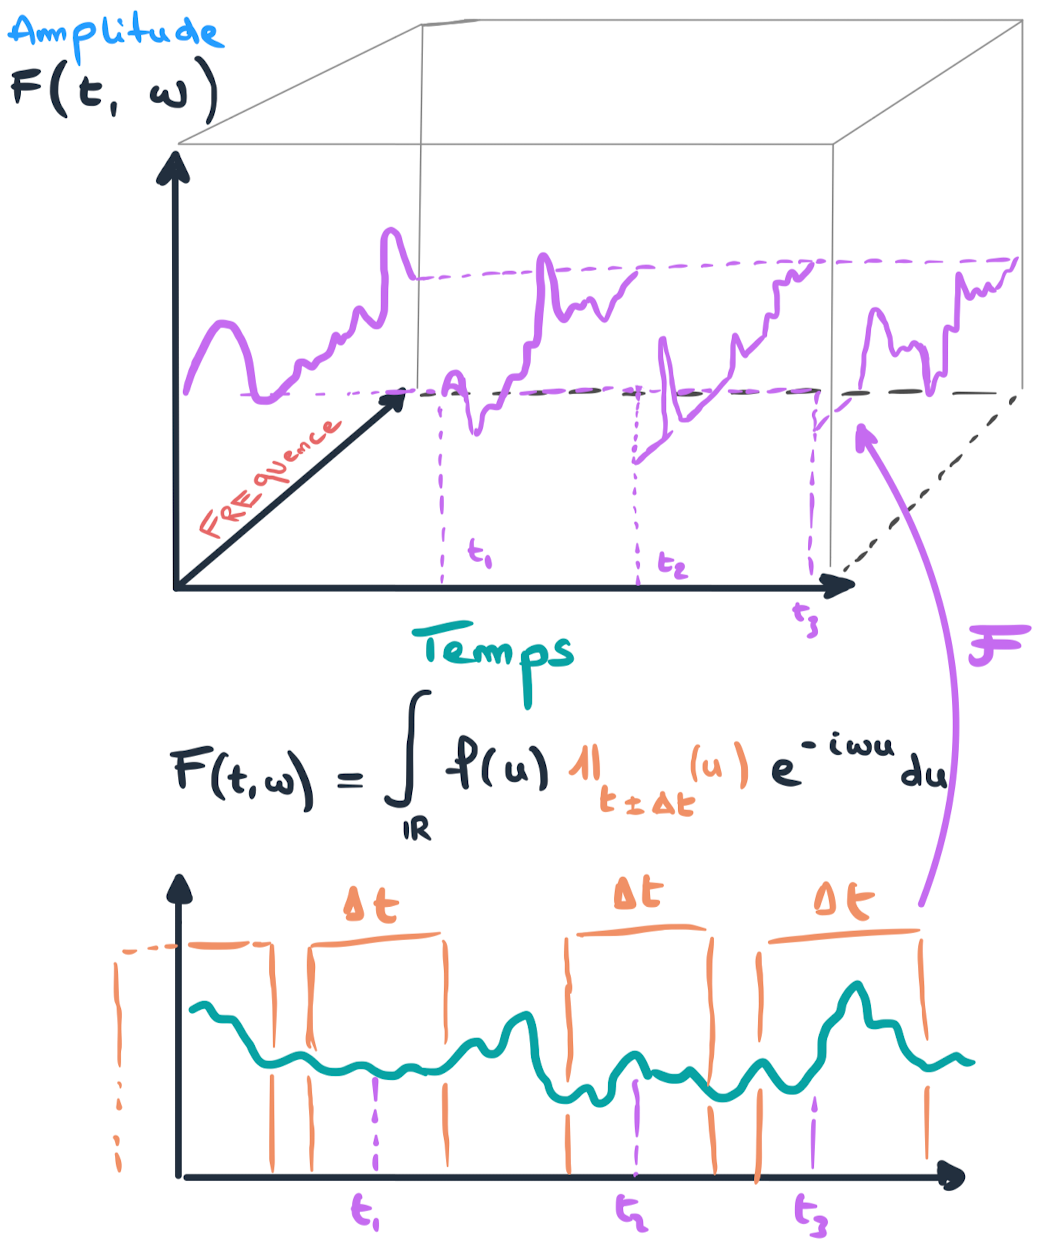
\includegraphics[width=\textwidth]{images/sketches/STFT.png}
        \caption{Transformée de Fourier à court terme d'une fonction}
        \label{fig:STFT}
    \end{figure}
\end{minipage}
\hfill
\begin{minipage}{0.60 \textwidth}
 
    Cependant contrairement à ce que peut suggérer le dessin présenté ici, la résolution fréquentielle n'est pas parfaite. Elle est d'ailleurs dans le cadre de la Transformée de Fourier à court terme constante, que ce soit sur le domaine temporel ou le domaine fréquentiel. La résolution fréquentielle est donc constante quelque soit la fréquence considérée.

    \question{
        \smallskip\centering
        Quel est le problème avec cette approche ?
    }

    le problème ne vient pas du monde mathématique mais plutôt du monde réel : les signaux que l'on observent présentent la caractéristique suivante : Les signaux de basse fréquence ont tendance à s'étendre sur la durée, et les signaux de hautes fréquences ont tendance à être très localisées, sous forme d'impulsion. Il devient alors clair que pour correctement identifier et localiser les fréquences présentes dans un signal, il est judicieux (voire parfois nécessaire) de varier la résolution fréquentielle et temporaire (limitées par le théorème d'indétermination de Heisenberg) en fonction de ce qui est le plus difficile à distinguer. C'est ce que proposent les ondelettes.
    
\end{minipage}

\subsubsection{Théorie de la base ondelettes}

\textbf{Transformée en ondelettes}

Introduisons maintenant de façon plus formelle les ondelettes et regardons leurs propriétés intéressantes dans le cadre du lissage de trajectoires.

on définit la transformée en ondelettes vis à vis de l'ondelette mère $\psi$ d'une fonction $f$ par :

$$F : \begin{array}{ccc}
  \mathds R \times \mathds R_+  &\longrightarrow & \mathds R
    \\
   (t,s) & \longmapsto & \displaystyle\frac 1 { \sqrt{|s|}} \int_{\mathds R} f(\colorize{u}) \psi \left( \frac{\colorize{u}-t}{s} \right) \mathrm d \colorize{u}
\end{array}$$

\brain{on peut remarquer que la formule de la transformée en ondelettes ressemble à une projection : $\displaystyle\frac{\langle f, \psi_{t,s} \rangle_{\mathds L^2}}{|| \psi_{t,s} ||}$. Cela vient en quelque sorte motiver la section suivante}

\textbf{Base d'ondelettes}

$$
\left( \psi_{k,n} : t \mapsto \frac 1 {\sqrt{2^k}} \psi( \frac{t - 2^k n}{2^k} ) \right)_{(k,n) \in \mathds Z^2} \textsf{ est une base } \vcenter{\hbox{$\underset{\| \cdot \|}{\perp}$}} \textsf{ de } \mathds L^2
$$
 
\info{notons que les résolutions sont des puissances de 2, ceci est un détail qui demandera une implémentation particulière dans le cadre des données réelles : il faudra faire attention à ce que le nombre de points que l'on donne dans l'algorithme de transformée rapide en ondelettes soit aussi une puissance de 2.}

\textbf{Propriétés principales des ondelettes}

\smallskip

\begin{itemize}
    \item \textbf{Approximation dans l'espace fréquentiel-temporel} : La transofrmée en ondelettes ( $\mathcal W : f \mapsto \langle f \, | \, \psi_{t,s} \rangle$ ) est une isométrie de $\mathds L^2$. Cela nous permet donc d'affirmer que $|| f - \hat f ||_{\mathds L^2} = || \mathcal W f - \mathcal W \hat f ||_{\mathds L^2}$. Ainsi on peut travailler dans l'espace des ondelettes pour approximer (dans notre cas lisser les trajectoires) des fonctions et contrôler l'approximation directement dans le domaine fréquence-temporel tout en le conservant dans le domaine temporel. \citationrequise
    % @ todo : compléter citation — STFT : talk de Stéphane Mallat

    \item \textbf{Propriété de Fast Decay}
\end{itemize}



\subsubsection{Motivation dans le cadre de l'analyse de données fonctionnelles}

\subsubsection{Effets du lissage à ondelettes sur la régularité locale}



\section{Estimation adaptative}

\subsection{Estimation adaptative de la fonction moyenne}



L'idée du lissage adaptatif est que chaque quantité évaluée en un point $t \in \mathcal T$ tire parti différemment des information du voisinage de $t$. Il semble intuitif que le processus moyen ($\mu = \esperance{X}$) considère des informations d'un voisinage assez large du processus et que celui-ci soit \og assez lisse \fg. Pour déterminer une fenêtre adaptée à l'estimation de la moyenne, on définit une grille de fenêtres à évaluer $\mathfrak H = (h_i)_{1:r}$ que l'on choisit en minimisant un risque spécifiquement adapté :

\begin{equation*}
	\widehat{ h_\mu^* } = \argmin\limits_{h \in \mathfrak H} R_\mu( \, t \, , h \, )
\end{equation*}

\noindent Déterminons maintenant ce risque.

\subsubsection{Méthode Golovkine et al. : indépendance}

Dans le cadre de données indépendantes, on peut invoquer la Loi des Grands Nombres pour approximer l'espérance par la moyenne empirique.
On effectue une suite d'approximations de la façon suivante :

\begin{figure}[H]
	\centering
	\begin{tikzcd}[column sep=6cm, row sep=2cm]
		\widetilde{\mu_{\mathcal W}} \arrow[r, "\textsf{absence points } \mathcal W"] &\widetilde{\mu} \arrow[d, "LGN"]
		\\
		\widehat \mu \arrow[u, "\textsf{biais } \mathds B"] & \mu
	\end{tikzcd}
	\caption{Schéma du découpage du contrôle des erreurs}
\end{figure}

On détermine alors fenêtre de lissage en minimisant le risque suivant \cite{golovkine2021adaptive} :

\begin{equation*}
	R_\mu^{[Golovk.]}(t, h) = \underbracket{q_1^2 h ^{2H_t}}_{\textsf{contrôle du biais}} +
	\underbracket{\frac{q_2^2}{\mathcal N_\mu(t, h)}}_{\textsf{contrôle de la variance}} +
	\underbracket{q_3^2 \bigl[ \frac{1}{\sum_k w_k} - \frac 1 n \bigr]}_{\textsf{pénalise absence de points}}
\end{equation*}

\info{
	Il est tout à fait  possible de regarder directement l'erreur d'approximation entre $\widetilde{\mu_{\mathcal W}}$ et $\mu$. Toutefois, le choix de Golovkine est avant tout un choix pédagogique, pour signaler et renforcer l'idée qu'il faut faire attention à l'erreur d'approximation entre l'inobservable et le véritable processus ( $\mathds E \, X$ vs $\frac 1 N \sum X_i \neq \frac 1 N \sum \widehat X_i$)
}

Afin de prendre en compte la dépendance, que l'on doit contrôler aussi, on raisonne plutôt de la façon suivante.

\subsubsection{Méthode MPV : dépendance}

Lorsque l'on traite le cas de la dépendance, il est tout de suite plus délicat d'obtenir la convergence d'estimateurs de moments d'une loi. MPV utilise ce découpage du risque pour déterminer une fenêtre de lissage adaptée à l'estimation de la fonction moyenne :

\begin{figure}[H]
	\centering
	\begin{tikzcd}[column sep=6cm, row sep=2cm]
		\widetilde{\mu_{\mathcal W}} \arrow[r, "\textsf{absence points } \mathcal W", color=flatuicolors_light_gray] \arrow[dr, "\textsf{MPV : absence points } P_N + \textsf{ dépendance } \mathds D", flatuicolors_green, sloped] &\widetilde{\mu} \arrow[d, "LGN", color=flatuicolors_light_gray]
		\\
		\widehat \mu \arrow[u, "\textsf{biais } \mathds B"] & \mu
	\end{tikzcd}
	\caption{Schéma du découpage du contrôle des erreurs}
\end{figure}

On détermine cette fois-ci la fenêtre de lissage en minimisant le risque suivant \cite{maissoro-SmoothnessFTSweakDep} :

\begin{equation*}
	R_\mu( \, t \, , h \, ) =
	\underbracket{L_t^2 h ^{2H_t} \mathds B( \, t, h, 2H_t \,) }_{\textsf{contrôle du biais}}
	+ \underbracket{\sigma^2 \mathds V_\mu( \, t, h \, ) }_{\textsf{contrôle de la variance}}
	+ \underbracket{\frac{\mathds D_\mu( \, t \, )}{P_N(t, h)}}_{\textsf{contrôle de la dépendance}}
\end{equation*}






\subsection{Estimation adaptative de l'opérateur de covariance}

On souhaite désormais estimer la quantité la covariance de la loi de notre processus. Si il semblerait naturel d'évaluer :

\begin{equation*}
	C_X(s,t) = \esperance{ \bigl(X(t) - \mu(t)\bigr) \cdot \bigl( X(s) - \mu(s) \bigr) }
\end{equation*}

la quantité qui nous intéresse, in-fine est l'opérateur de covariance :

\begin{equation*}
	c[ \, f \,] = \int_I f(u)c(u, \, \cdot \, ) \, du
\end{equation*}

C'est parceque c'est cet opérateur qui nous donnera, notamment, les vecteurs et valeurs propres de la décomposition dans la base FPCA, aussi connue sous le nom de décomposition de Karhunen-Loève.

\bigskip

On comprend bien que la covariance est une quantité qui mesure la dispersion des données et qu'il est donc naturel de s'intéresser beaucoup plus aux fines variations dans un voisinage proche du couple $(t,s)$ des différents temps qui nous intéressent. Cela vient motiver, une fois de plus l'intérêt de l'utilisation d'un lissage adaptatif qui nous est donné par la minimisation du risque suivant ~\cite{maissoro-SmoothnessFTSweakDep} :

\begin{equation*}
	R_\Gamma( t, h ) =
\end{equation*}

\subsection{Estimation adaptative de l'auto-covariance des séries temporelles fonctionnelles}

\input{content/chapter_2/estimation_adaptative__autocovariance.tex}